\section{Hand Dimensionality}

At the core of our technique is the assumption that hand motion is
relatively low-dimensional.  Even though a full resolution skeleton
of the hand can have several dozen degrees of freedom (DOF),
many of the DOFs of the hand are dependent~\cite{SanFlaSoe98,BraZha04,JoeOSu09}. 
In our approach, we exploit this low dimensionality through PCA, assuming that PCA
will capture the important features of the whole-body hand
in a relatively small number of principle components. 
Further, we assume that
if we record markers that well-inform these \emph{key} principle components, we can estimate the
DOFs of the whole hand.  

To support these assumptions, we performed various tests to tease out the power of
PCA our testbed for hand animation.
Starting from a reference database, we conduct PCA to produce a new representation
of the data.  
%
%We experimented with two ways to construct 
%the joint angles from the 
%marker database.
%
Specfically, PCA is performed 
over the joint angles, giving us a new principle component 
representation of the joints angles with 54 components (assuming a skeleton of 18~joints,
with 3 Euler angles each). 
%for every sample of motion in the database.  
%
We performed an analysis to judge the ability of the PCA to directly 
reconstruct the original database motion and found that with as few as ten 
components the PCA could produce a motion with small but acceptable 
visual artifacts.  An error plot of the reconstruction error measured by the
joint angle deviation from the synthesized motion and the original motion
appears in Figure~\ref{BLAH}.  Similar findings are reported using a small
set of components from PCA to
encapsulate the motion of full-body motion in~\cite{Alla} and our results
here support similar observations made over hand data.

We also used PCA on the marker positions of the samples appearing in 
the reference database.  The dimensionality of this PCA representation
is 39, comprised of 3 root-corrected position values for each of the 13 markers.  

We support this primary assumption by showing that joint angles alone
are not capable of producing the reconstructions we realize through PCA in Figure~\ref{}. 

\begin{figure}[ht]
  \centering
  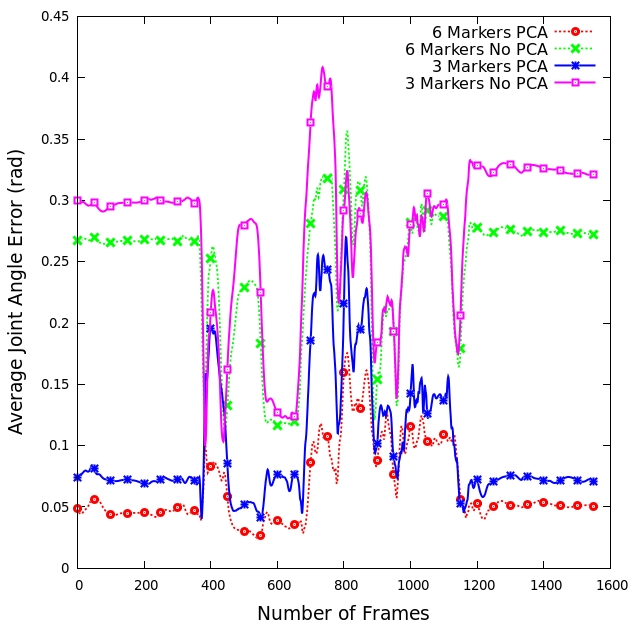
\includegraphics{images/avgError_6_3_jangles_babySigns1.jpg}
  \caption{PCA vs. Joint angles.}
\end{figure}

  components that 
sample in the database. PCA identifies the most important information 
in this database by making it the first component. Each subsequent 
component is less valuable than its predecessor. Using this knowledge, 
we sum up the values of each component over all of the samples and 
weigh each sum based on importance (which component). Each weighted 
sum correlates with a marker, and the markers are then ordered in terms 
of importance by their weighted sum. The chosen marker set is then 
used for the data we wish to reconstruct. \\

To reconstruct a sequence of motion, we first only use data from the 
marker set selected in the previous step. This is the equivalent of 
having our performer only wear these markers in the initial capture 
session. These marker position are plugged into our regression model 
to determine the full motion of our low dimensional sequence in 
principle component space. \\

%Using PCA, we can also construct an optimal marker set to represent our 
%low dimensional data. 


